%
% This is the LaTeX source for the notes of Lecture 1; please use this as a
% template file for your scribe notes, and follow its style as far as possible.
%

\documentclass[twoside]{article}
\usepackage{graphicx} 
\usepackage{amsmath,tikz,amsfonts,amssymb,multicol}
\setlength{\oddsidemargin}{0.25 in}
\setlength{\evensidemargin}{-0.25 in}
\setlength{\topmargin}{-0.6 in}
\setlength{\textwidth}{6.5 in}
\setlength{\textheight}{8.5 in}
\setlength{\headsep}{0.75 in}
\setlength{\parindent}{0 in}
\setlength{\parskip}{0.1 in}


%
% The following commands set up the lecnum (lecture number)
% counter and make various numbering schemes work relative
% to the lecture number.
%
\newcounter{lecnum}
\renewcommand{\thepage}{\thelecnum-\arabic{page}}
\renewcommand{\thesection}{\thelecnum.\arabic{section}}
\renewcommand{\theequation}{\thelecnum.\arabic{equation}}
\renewcommand{\thefigure}{\thelecnum.\arabic{figure}}
\renewcommand{\thetable}{\thelecnum.\arabic{table}}

%
% The following macro is used to generate the header.
%
\newcommand{\lecture}[4]{
   \pagestyle{myheadings}
   \thispagestyle{plain}
   \newpage
   \setcounter{lecnum}{#1}
   \setcounter{page}{1}
   \noindent
   \begin{center}
   \framebox{
      \vbox{\vspace{2mm}
    \hbox to 6.28in { {\bf CS 7535~Markov Chain Monte Carlo Methods
                        \hfill Fall 2017} }
       \vspace{4mm}
       \hbox to 6.28in { {\Large \hfill Lecture #1: #2  \hfill} }
       \vspace{2mm}
       \hbox to 6.28in { {\it Lecturer: #3 \hfill Scribes: #4} }
      \vspace{2mm}}
   }
   \end{center}
   \markboth{Lecture #1: #2}{Lectures #1: #2}
   {\bf Disclaimer}: {\it These notes have not been subjected to the
   usual scrutiny reserved for formal publications.  They may be distributed
   outside this class only with the permission of the Instructor.}
   \vspace*{4mm}
}

%
% Convention for citations is authors' initials followed by the year.
% For example, to cite a paper by Leighton and Maggs you would type
% \cite{LM89}, and to cite a paper by Strassen you would type \cite{S69}.
% (To avoid bibliography problems, we redefine the \cite command.)
% Also commands that create a suitable format for the reference list.
\renewcommand{\cite}[1]{[#1]}
\def\beginrefs{\begin{list}%
        {[\arabic{equation}]}{\usecounter{equation}
         \setlength{\leftmargin}{2.0truecm}\setlength{\labelsep}{0.4truecm}%
         \setlength{\labelwidth}{1.6truecm}}}
\def\endrefs{\end{list}}
\def\bibentry#1{\item[\hbox{[#1]}]}

% Use these for theorems, lemmas, proofs, etc.
\newtheorem{theorem}{Theorem}[lecnum]
\newtheorem{lemma}[theorem]{Lemma}
\newtheorem{proposition}[theorem]{Proposition}
\newtheorem{claim}[theorem]{Claim}
\newtheorem{corollary}[theorem]{Corollary}
\newtheorem{definition}[theorem]{Definition}
\newenvironment{proof}{{\bf Proof:}}{\hfill\rule{2mm}{2mm}}

% **** IF YOU WANT TO DEFINE ADDITIONAL MACROS FOR YOURSELF, PUT THEM HERE:
\DeclareMathOperator{\sgn}{sgn}
\DeclareMathOperator{\contrib}{contrib}

\begin{document}
%FILL IN THE RIGHT INFO.
%\lecture{**LECTURE-NUMBER**}{**DATE**}{**LECTURER**}{**SCRIBE**}
\lecture{1}{August 22}{Prof. Eric Vigoda}{Sam Seifert}

% **** YOUR NOTES GO HERE:

%**** IN GENERAL, BE BRIEF. LONG SCRIBE NOTES, NO MATTER HOW WELL WRITTEN,
%**** ARE NEVER READ BY ANYBODY.


\lecture{2}{August 24}{Prof. Eric Vigoda}{Tim Duff}

Let $G$ be an undirected graph with vertex set $[n] := \{ 0, 1, \ldots , n-1 \}$ and $\mathcal{P}$ denote the set of all perfect matchings in $G.$ We would like an an algorithm, polynomial in $n,$ for computing $|\mathcal{P}|.$ This is ``hard'' to compute exactly for general graphs, but attainable when $G$ is \emph{planar.} Last time, we gave an algorithm due to Kasteleyn which takes a plane-embedded graph and outputs a \textbf{Pfaffian orientation}---that is, an orientation $\vec{G}$ such that for all $P,P'\in \mathcal{P},$ every even cycle in $P\cup P'$ has an odd number of edges opposite of its traverse sequence (see Figure~\ref{pfaff_pic}.)
\begin{figure}
\begin{center}
\begin{multicols}{2}
%undirected


\begin{tikzpicture}{rotate=90}
\node[fill=black] (v1) at (0,0) {};
\node[fill=black] (v2) at (1,0) {};
\node[fill=black] (v5) at (0,1) {};
\node[fill=black] (v6) at (1,1) {};
\draw[line width=0.55mm] (v1) -- (v2);
\draw[line width=0.55mm] (v6) -- (v5);
\draw[line width=0.55mm] (v6) -- (v2);
\draw[line width=0.55mm] (v1) -- (v5);
\draw[line width=0.55mm] (v1) -- (v6);
\end{tikzpicture}

\columnbreak 


%directed
\begin{tikzpicture}{rotate=90}
\node[fill=black] (v1) at (0,0) {};
\node[fill=black] (v2) at (1,0) {};
\node[fill=black] (v5) at (0,1) {};
\node[fill=black] (v6) at (1,1) {};
\draw[line width=0.55mm, blue, ->] (v1) -- (v2);
\draw[line width=0.55mm, blue, ->] (v6) -- (v5);
\draw[line width=0.55mm, red, ->] (v6) -- (v2);
\draw[line width=0.55mm, red, ->] (v1) -- (v5);
\draw[line width=0.55mm, black, ->] (v1) -- (v6);
\end{tikzpicture}
\end{multicols}
\end{center}
\caption{Non-Pfaffian orientation.}
\label{pfaff_pic}
\end{figure}


Given a Pfaffian orientation $\vec{G},$ consider the $n\times n$ skew-symmetric adjacency matrix defined by
\[
\vec{A}[i,j] = \begin{cases}
\,  \, \, \, \, 1 \indent  \, \, \, \text{ if } \indent  \overrightarrow{i\, j}\in E(\vec{G}), \\
-1 \indent \, \, \,  \text{ if }  \indent \overrightarrow{j\, i} \in E(\vec{G}),\\
\, \, \, \, \, 0  \, \, \, \indent \text{ else.}
\end{cases}
\]
The following theorem, paired with Kastelyn's algorithm and a linear-time planar embedding algorithm, shows that the problem of counting perfect matchings in planar graphs is in $\mathbf{P}.$
\begin{theorem}
If $\vec{G}$ is Pfaffian, then $\det \vec{A}= |\mathcal{P}|^2.$ 
\end{theorem}
\begin{proof}
Construct a digraph $D=([n],A),$ where $A$ consists of each edge in $G$ in either possible orientation. We begin by showing that
\[
|\mathcal{E}| = |\mathcal{P}|^2,
\]
where $\mathcal{E}$ is the set of even cycle covers in $D.$\footnote{For us an \textbf{even cycle cover} of $D$ is a collection of vertex-disjoint directed cycles of even length in $D$ such that each vertex of $D$ is contained in a cycle.} Noting the natural ordering on $[n],$ consider the map $f: \mathcal{P} \times \mathcal{P} \rightarrow \mathcal{E}$ which takes a pair $(P,P')$ and directs each cycle $C\subset P\cup P'$ starting from the lowest vertex present (say $i$) to its unique $C$-neighbor (say $j$) such that $ij \in P.$ To see that $f$ is invertible, fix a cycle cover in $\mathcal{E}.$ We may order the edges of any cycle appearing in this cover as $\overrightarrow{i_1 i_2}, \,  \ldots ,  \, \overrightarrow{i_L i_1} $ with $i_1$ minimal---with this ordering scheme, $f^{-1}$ takes our cycle cover to the pair (``odd edges'', ``even edges'') $\in \mathcal{P}.$\\\\
We may now evaluate the determinant
\[
\det \vec{A} = \displaystyle\sum_{\sigma \in S_n} \sgn  \sigma \, \displaystyle\prod_{i\in n} \vec{A} [i,  \sigma (i)]
\]
by taking an arbitrary permutation with cycle decomposition $\sigma = \gamma_1 \, \cdots \, \gamma_k$ and finding its contribution to the sum by considering cases:
\begin{itemize}
\item[1)] If $\sigma $ has a cycle of odd length, let $\gamma_i$ denote the leftmost one and define $\sigma ' = \gamma_1 \, \cdots \, \gamma_{i-1} \, \gamma_i^{-1} \, \gamma_{i+1} \, \cdots \, \gamma_k.$ We have that
\[
\sgn \sigma = (-1)^{n-k} = \sgn \sigma ' \, \, \text{ and } \, \, \displaystyle\prod_{i\in n} \vec{A} [i,  \sigma ' (i)] = (-1) \times \displaystyle\prod_{i\in n} \vec{A} [i,  \sigma (i)].
\]
Thus, noting $\sigma '' = \sigma ,$ the total contribution from such $\sigma $ is zero.
\item[2)] For the case where all cycles in $\sigma $ have even length, the product 
\[
\prod_{i\in [n]} \vec{A}[i,\sigma (i)] \label{eq:match_prod} \tag{*} 
\]
is nonzero iff the $\gamma_i$ determine a cycle cover for $D.$ Here, we use the fact that the orientation is Pfaffian. Each directed cycle corresponding to $\gamma_i$ in turn corresponds to an even cycle formed by the union of two perfect matchings in $G$---since $\vec{G}$ oddly orients this cycle, we see that each $\gamma_i$ contributes $-1$ to the product~\eqref{eq:match_prod}. Now
\[
\sgn \sigma \times \displaystyle\prod_{i=1}^k \contrib (\gamma_i) = (-1)^{n-k} \times (-1)^k = (-1)^n,
\]
gives a total contribution of $(-1)^n \, |\mathcal{E}| = |\mathcal{E}|,$ the last equality being clear for $n$ even and trivial for $n$ odd, since then $|\mathcal{E}|=0.$
\end{itemize}
\end{proof}



% **** THIS ENDS THE MAIN TEXT.  DON'T DELETE THE FOLLOWING LINE:
\section*{References}
\beginrefs


\bibentry{MRST97}
{\sc W.~Mccuaig}, {\sc N.~Robertson}, {\sc P. Seymour} and {\sc R.~Thomas},
`Permanents, Pfaffian orientations, and even directed circuits,''
{\it Proceedings of the 29th ACM STOC}, 1997, pp.~402--405.


\bibentry{L02}
{\sc J.~Liu},
{\it Monte Carlo Strategies in Scientific Computing},
Springer, 2002.

\bibentry{TF61}
{\sc H.~N.~V.~Temperly} and {\sc M.~E.~Fischer}.
``Dimer problem
in statistical mechanics---an
exact result,''
{\it Philosophical Magazine} \textbf{6(68)} (1961), pp.~1061--1063.


\endrefs

\end{document}





